% sim_detach.tex -- Results: detach in simulation (draft 4 Oct 2026). No run ids in the text.
% Runs: OCP vs network R0111-R0114 (6 Aug, 0.4 kg payload, 0.5 m cables, circle 0.6 m/s);
% hand-back R0093 (even ring, 62 deg), R0108/R0109; SIL mode study R0496-R0505 (25 Sep);
% layout R0559-R0572 (hover) and R0554/R0556 (mid-circle) (25 Sep, legacy
% linear plant, 0.86 kg ring, 0.5 m rods, 0.64 kg UAVs); 1/3/6/9 R0582/R0584; LAND v4 R0571/R0572;
% rig twin W4 rehearsal R0939 (4 Oct, 0.55 m rods, 0.55 kg UAVs, affine map, old tracker box).
% Restructured 9 Oct (structure audit): opens with its question, baseline and bar; order layout,
% transient, against the network, rig; the freed UAV's own landing added (fig:departed_landing) with
% pending rig figures.

\subsection{Detach}
\label{sec:sim_detach}

This section answers the leave half of RQ1: does a detach by OCP resize keep the ring level when one UAV
of four leaves? The baseline is a hand-off of the payload to the dissipative network on the same
detach, and for the geometry the even layout; the bar is the ring's tilt back under the hover's own
maximum plus 0.5$^\circ$ (Table~\ref{tab:detach}).

\paragraph{Layout.}
\redo{detach layout study, four UAVs to three in hover, the UAV on plate~3 released, two runs per layout: the even ring (plates 0/3/6/9) against plates 1/3/5/9 (peak and settled tilt); the 1/3/5/9 detach in the middle of a circle; plates 1/3/6/9 (clearance of the departing UAV against tilt and throttle).}
% --- original text, flown before the rig twin; kept to refill this place:
% \paragraph{Layout.} The geometric condition of Section~\ref{sec:reconfig} was tested directly. Four
% UAVs on an even ring (plates 0/3/6/9) and on plates 1/3/5/9 hovered, and the UAV on plate~3 was
% released. On the even ring the three survivors' attachment points have the ring's centre of mass on
% the edge of their support triangle, and the payload swung to a 25.6--28.5$^\circ$ peak and settled at
% 6.7--6.8$^\circ$. On plates 1/3/5/9 the survivors form an even triangle: the peak was
% 3.0--3.3$^\circ$ and the payload settled at 0.1--0.2$^\circ$ (Table~\ref{tab:detach_layout}). The same
% detach in the middle of a circle peaked at 6.9--7.7$^\circ$ and settled at 0.3$^\circ$, and the
% survivors continued the circle. Moving one more UAV, to plates 1/3/6/9, gives the departing UAV more
% room (0.82\,m to its nearest neighbour instead of 0.58\,m) at a cost of 2.5$^\circ$ of peak tilt,
% 0.45$^\circ$ of settled tilt and 10\,\% more throttle on one survivor.
%
% \begin{table}[h]
% \centering
% \caption{Detach from four UAVs to three in hover, Gazebo, 0.86\,kg ring, by layout. Two runs per layout.}
% \label{tab:detach_layout}
% \begin{tabular}{lcc}
% \toprule
% Layout (plates) & Peak tilt after DETACH & Settled tilt \\
% \midrule
% Even, 0/3/6/9 & 25.6--28.5$^\circ$ & 6.7--6.8$^\circ$ \\
% 1/3/5/9 & 3.0--3.3$^\circ$ & 0.1--0.2$^\circ$ \\
% 1/3/5/9, mid-circle & 6.9--7.7$^\circ$ & 0.3$^\circ$ \\
% \bottomrule
% \end{tabular}
% \end{table}

\paragraph{The transient.} Figure~\ref{fig:detach} shows one detach in the rig twin: four UAVs on plates 1/3/5/9 in hover, the
UAV on plate~3 released, with $\epsilon = 0$. The uneven 1/3/5/9 layout loads the UAV on plate~9 most.
At DETACH the planner, re-solved for the three survivors on their actual plates, hands the released
UAV's load to them in one 0.1\,s tick. The ring tilts by at most 3.3$^\circ$ and is back within its
hover band after 1\,s.

\begin{figure}[h]
\centering
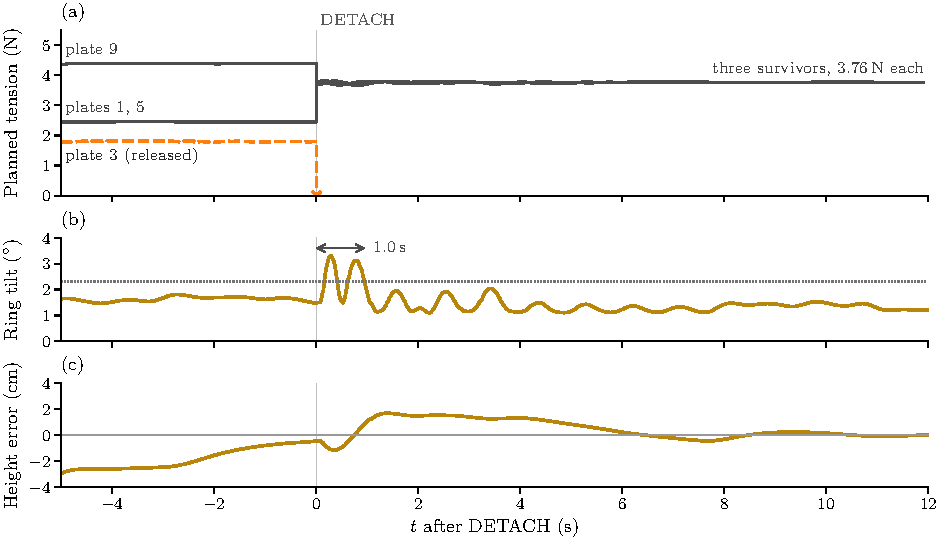
\includegraphics[width=\textwidth]{Images/detach.pdf}
\caption[Detach by OCP resize]{Detach of one UAV of four by OCP resize, Gazebo rig twin, hover at
1.0\,m, UAVs on plates 1, 3, 5 and 9 (Figure~\ref{fig:geometry}). (a) Rod tension planned for each
UAV; the UAV on plate~3 (dashed) is released at DETACH, and the three survivors, now an even
triangle, share the load equally. (b) Ring tilt; dotted: the hover's own maximum plus 0.5$^\circ$;
arrow: time until the tilt stays below it. (c) Ring height error against the 1.0\,m target. One run;
the tensions are planned, since the rig twin does not measure them.}
\label{fig:detach}
\end{figure}

\paragraph{Repeats.} Table~\ref{tab:detach} gives the same detach over five runs with $\epsilon = 0$,
against the earlier rehearsal, which differed in two ways: the relaxed box and the height integral on.
With $\epsilon = 0$ every run peaks at a few degrees and is back within its hover band in about a
second, and the five runs agree closely.

\begin{table}[htbp]
\centering
\caption[Detach, repeats]{Detach of one UAV of four in hover by OCP resize, Gazebo rig twin, plates 1,
3, 5 and 9, ring at 1.0\,m. Peak tilt: in the 5\,s after DETACH. Back in band: time until the tilt
stays under the hover's own maximum plus 0.5$^\circ$. Height change: largest change from the mean
height before DETACH, in the 12\,s after. Ranges over the runs.}
\label{tab:detach}
% generated by tools/thesis_sim_tables.py
\begin{tabularx}{\textwidth}{>{\raggedright\arraybackslash}Xcccc}
\toprule
 & & Peak tilt & Back in band & Height change \\
Tracker box & Runs & (\si{\degree}) & (s) & (cm) \\
\midrule
$\epsilon = 0.025$, height integral on & 1 & 3.2 & 2.6 & 2.7 \\
$\epsilon = 0$, no integral & 5 & 2.8--4.0 & 0.9--1.0 & 3.4--3.6 \\
\bottomrule
\end{tabularx}

\end{table}

\paragraph{OCP resize against network hand-off.}
\redo{OCP resize against network hand-off on the same detach, four UAVs to three during a circle (and in hover): settled payload tilt and the survivors' tracking error; with it the network's hand-back to the planner, with and without the two fixes (no soft-start restart on an airborne hand-back, solver primed before it flies).}
% --- original text, flown before the rig twin; kept to refill this place:
% \paragraph{OCP resize against network hand-off.} Table~\ref{tab:detach_ab} compares the two detach
% methods of Section~\ref{sec:reconfig} on the same flight: four UAVs flying a circle, one released
% mid-way. The flights used an early payload (0.4\,kg, 0.5\,m cables, circle at 0.6\,m/s). With the OCP
% resize the payload settled level and the survivors kept tracking their references. With the network
% hand-off the payload settled tilted by 26--48$^\circ$, and the survivors were 0.06--0.91\,m off their
% references while the network redistributed the load. Two fixes were needed for the network sequence
% to hand back to the planner at all: the feedforward soft-start must not restart on an airborne
% hand-back, and the new solver must be primed before it flies. Without them the payload dropped to
% 0.07\,m above the floor after the detach; with them it stayed above 0.46\,m.
%
% \begin{table}[h]
% \centering
% \caption{Detach from four UAVs to three during a circle, Gazebo, early payload (0.4\,kg).}
% \label{tab:detach_ab}
% \begin{tabular}{lcc}
% \toprule
%  & OCP resize & Network hand-off \\
% \midrule
% settled payload tilt & about 1$^\circ$ & 26--48$^\circ$ \\
% survivor tracking error & about 1\,mm & 60--910\,mm \\
% \bottomrule
% \end{tabular}
% \end{table}

\redo{the same comparison on a plant that matches the controller's model (the software-in-the-loop bench, once it flies the twin), hover and circle: payload tilt after the detach with the network against the OCP resize.}
% --- original text, flown before the rig twin; kept to refill this place:
% On the 0.86\,kg ring the gap widened. In the software-in-the-loop bench the network aborted the
% flight at 53--61$^\circ$ of payload tilt after a detach, both in hover and in the circle, while the
% OCP resize held the survivors level to within 0.5--2$^\circ$.

\paragraph{On the rig.} The detach was flown on the rig on 8 October, in four flights.
Figure~\ref{fig:rig_detach} sets their ring tilt and height error after the release against the twin.

\pendingfig{fig:rig_detach}{Detach on the rig against the twin: ring tilt and height error after the release for the announced, unannounced and 150-degree-gap detaches; rig gold, twin repeats grey.}{built from the 8 Oct rig runs (next)}

\paragraph{The freed UAV's own landing.} After a detach the freed UAV lands by itself, off the ring
(Section~\ref{sec:reconfig}). On the rig on 8 October this landing did not finish: in all four detach
flights the freed UAV floated above its resting height until the fleet's disarm at the end of the
landing dropped it about 0.3\,m (Figure~\ref{fig:departed_landing}a), and the twin shows the same stall
(Figure~\ref{fig:departed_landing}b). Its landing was therefore changed: its height reference is pushed
down to its own resting height, and once it is there it is disarmed alone, without waiting for the
fleet (Figure~\ref{fig:departed_landing}c, in the twin). Figure~\ref{fig:rig_departed} shows the
change on the rig.

\begin{figure}[htbp]
\centering
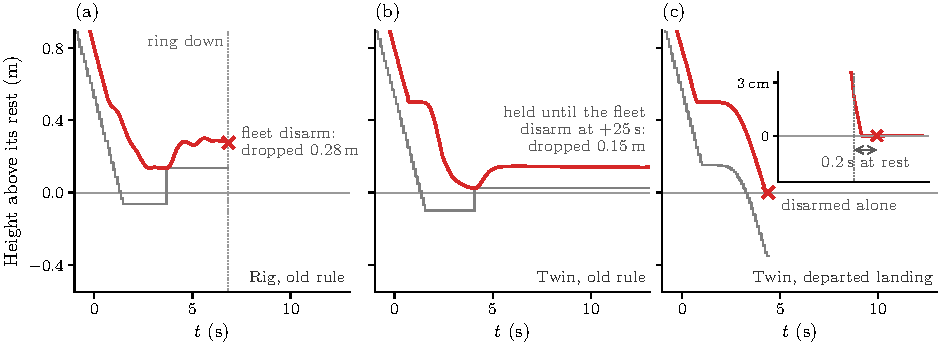
\includegraphics[width=\textwidth]{Images/departed_landing.pdf}
\caption[A freed UAV's own landing, old rule and departed landing]{A UAV landing by itself off the ring, the same UAV (QUAD4) in three cases, aligned where it passes 0.8\,m on the way down; solid: its height above its own resting height, grey: its height reference until it is disarmed, cross: its disarm, dotted: the ring reaching the floor. (a) Rig, old rule: its touchdown test fired 0.14\,m above its rest, the reference froze there, the UAV rose to 0.28\,m and hovered until the fleet's disarm at the end of the landing dropped it 0.28\,m. (b) Twin, old rule: the same stall, held 0.15\,m up for 25\,s until the fleet's disarm dropped it. (c) Twin, departed landing: the reference is pressed below the resting height until the UAV is there, and it is disarmed alone 0.2\,s after reaching it (inset). The plateau at 0.5\,m in (b) and (c) is the UAV standing on the tip of its rod before the rod tips over.}
\label{fig:departed_landing}
\end{figure}

\pendingfig{fig:rig_departed}{The freed UAV's own landing on the rig with the departed landing: pushed to its resting height and disarmed alone.}{rig W4/W5, 14 Oct}

\paragraph{Fewer than three.} Detaching from three UAVs to two is not attempted. A rigid payload on two
rim points is a pendulum about the line between them, and its centre of mass hangs off that line.
The planner refuses a detach that would leave fewer than three
UAVs.

\redo{a detach from three UAVs to two, to show the payload capsizing on two rim points.}
% --- original text, flown before the rig twin; kept to refill this place:
% In the bench the payload capsized. The planner refuses a detach that would leave fewer than three
